\section{Arkitektur}

\subsection{Systemarkitektur}
\noindent
Dette afsnit forklarer hvordan systemets toplevel arkitektur er opbygget.
Denne består af en bruger som interagerer med systemet gennem frontendapplikationen som skrives i WPF. States i denne applikation styres af Game modul som holder styr på hvor spilleren befinder sig, hvilke items der er samlet op og andre nyttige information som skal bruges gennem spillet.
Spillets backend benyttes primært til bruger authentication og som bindeled til databasen.
Databasen indeholder oplysninger om blandt andet brugere, de gemte spil og oplysninger om historien for de forskellige rum.
For at se en visuel repræsentation af hvordan de forskellige moduler snakker sammen se \autoref{fig:Arkitektur-SD-SaveGame}

\begin{figure}[H]
\centering
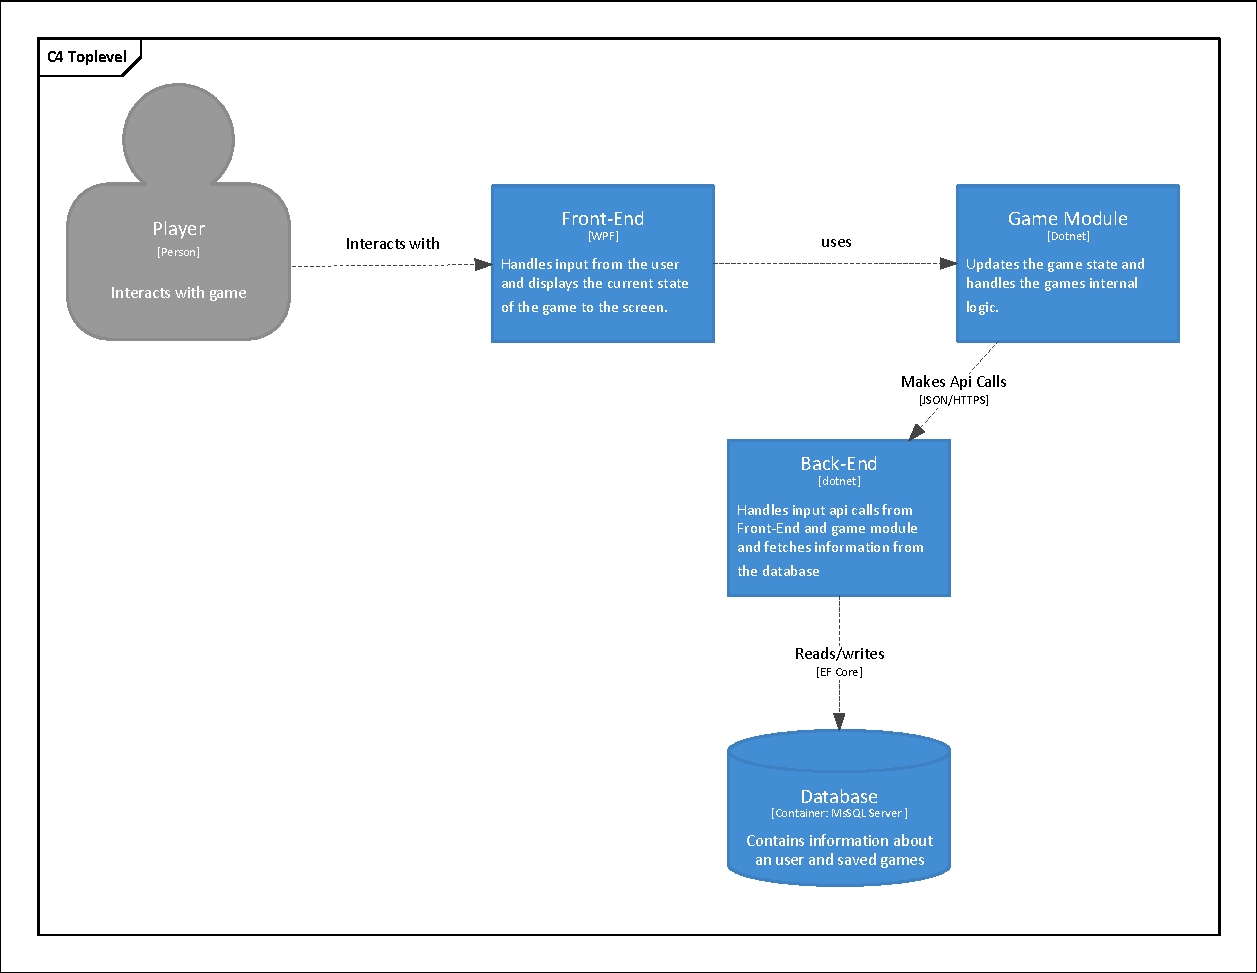
\includegraphics[width = \textwidth]{02-Body/Images/Arkitektur - C4TopLevel.pdf}
\caption{C4 Top-Level diagram for systemets arkitektur. Her ses et diagram for systemets Top-Level arkitektur, hvori der er skabt et overblik over hvilke moduler der er til stede i systemet og hvordan de kommunikere. Heri er der også tilføjet kommunikationsmetode for de forskellige forbindelser.}
\label{fig:Arkitektur-SD-SaveGame}
\end{figure}

\subsection{Frontend Arkitektur}

Frontend applikationen vil have til formål at håndtere brugerinput og output. Dvs. at der i Frontenden vises det data fra gamelogic, som brugeren skal have, og at det præsenteres på en overskuelig og brugervenlig måde. Dette resulterer i at brugeren kan forstå og kan finde ud af at bruge spillet på den tiltænkte måde.
Derudover skal Frontenden tage hånd om bruger input, og sørge for at brugeren giver korrekt input og at der tages hånd om eventuelt forkert input.\\
Da der er mange forskellige menuer og skærme i spil i frontenden er der lavet følgende C3 model for Frontenden (\autoref{fig:Arkitektur-FrontEnd-C3}), som giver en idé om hvilke skærme og menuer der kan gå til hvilke andre menuer/skærme. Udover dette fortæller modellen også om hvordan og hvilke skærme og menuer der snakker med noget uden for frontenden selv f.eks. skal der ved Login/Register kontaktes databasen for at få verificeret logind-oplysninger, og samtidig skal der ved save og load-game hentes en liste af gemte spil i databasen hvorefter der skal henholdsvis skrives og hentes fra databasen alt efter om man gemmer eller henter et spil. Der skal hertil nævnes at Login og Register står til at snakke med backenden direkte og ikke igennem gamelogic blokken, dette er valgt da funktionen ikke kaldes i gamelogic blokken, men den kaldes direkte i backend controlleren. Derudover er modellen mere overskuelig på denne måde og fungerer bedre til at give overblik over navigationen igennem menuerne.

\begin{figure}[H]
\centering
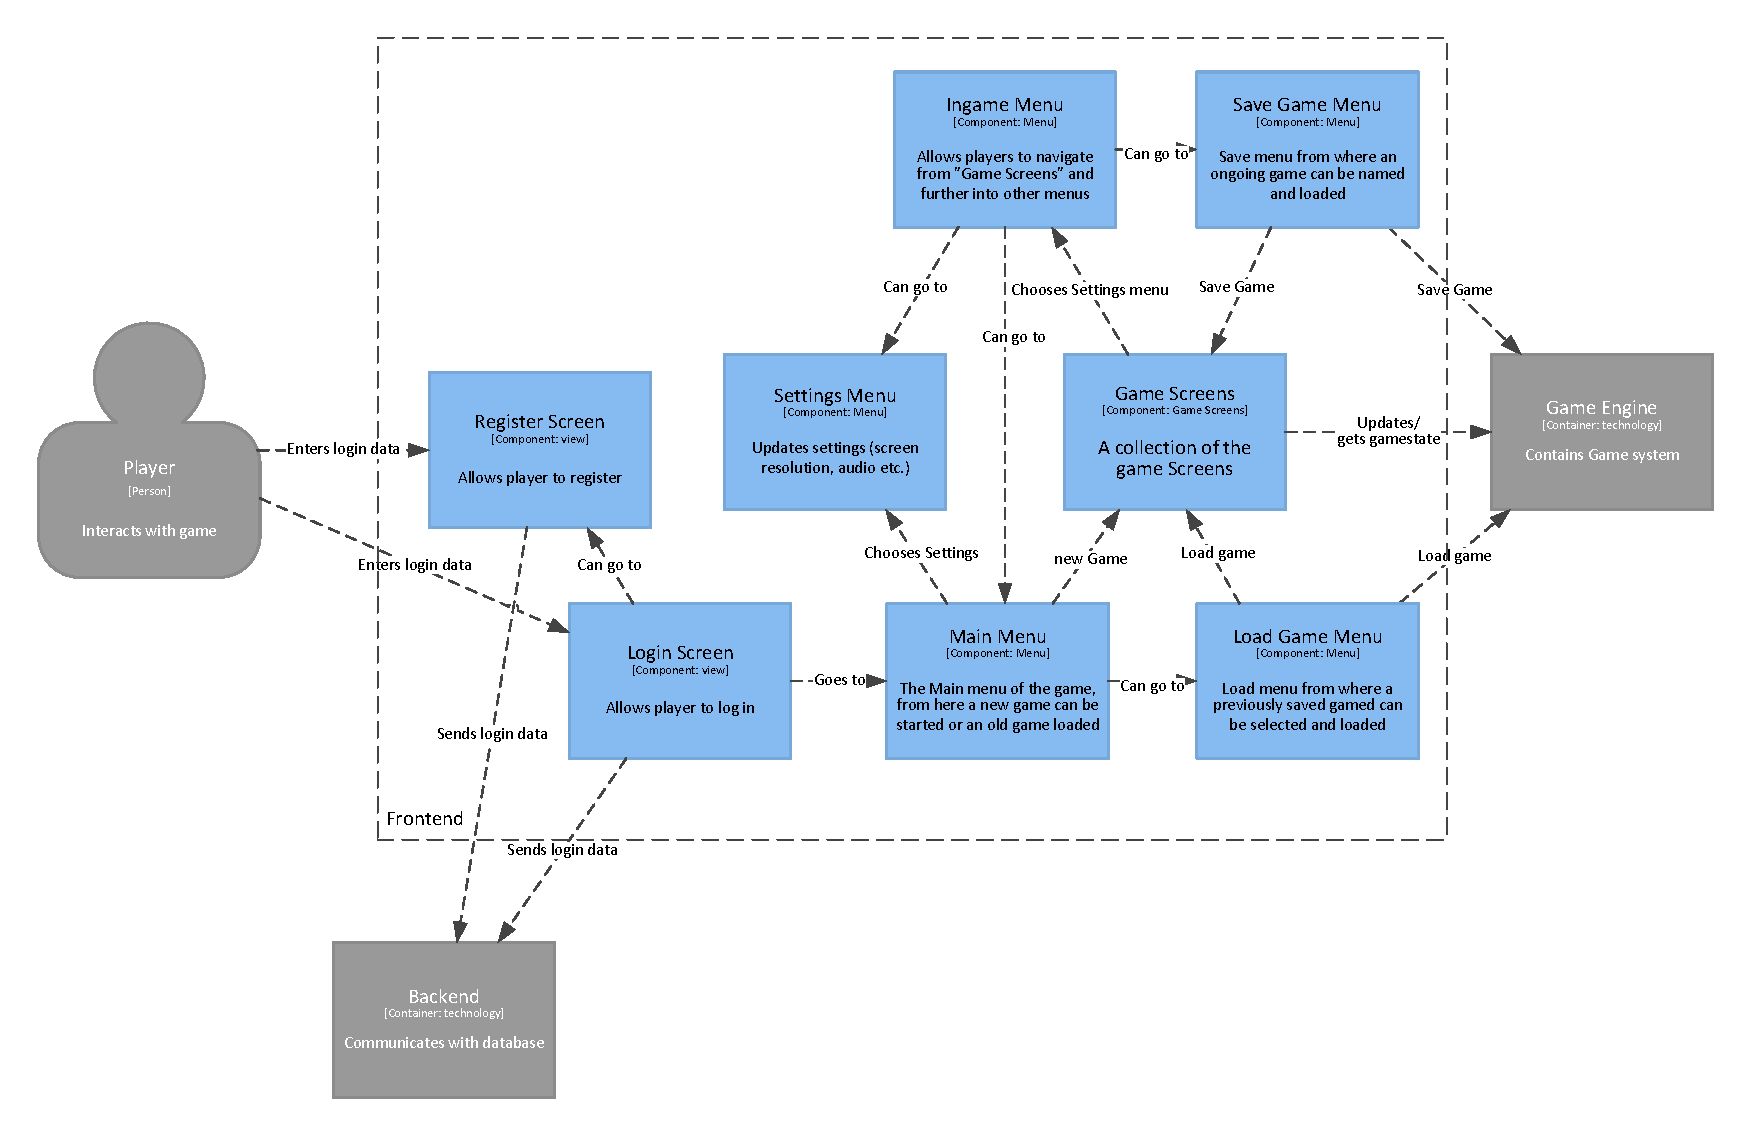
\includegraphics[width = \textwidth]{02-Body/Images/Frontend_C3.pdf}
\caption{C3-Model for Frontend. Modellen fortæller hvordan man kan navigere igennem forskellige menuer og hvilke menuer der kan føre til hvad. Derudover kan man se hvilke blokke der snakker ud af frontenden og sammen med resten af systemet.}
\label{fig:Arkitektur-FrontEnd-C3}
\end{figure}

\subsubsection{Pseudo Frontend Arkitektur}
(Hovedrapport stuff)
For at give overblik over, hvordan kommunikationen mellem frontend, backend og gamecontroller kommer til at foregå, er der lavet et pseudo sekvensdiagram for følgende UserStories:
\\
- Login\\
- Register\\
- Save Game\\
- Load Game\\
(/Hovedrapport stuff)
Der er ikke lavet sekvensdiagrammer for alle af projektets userstories, da mange af disse fungerer på samme måde og derfor ikke bidrager med noget nyt ift. dokumentationen.
Nedenfor ses pseudo sekvensdiagrammer for de fire userstories:\\
- Login\\
- Register\\
- Save Game\\
- Load Game\\

\noindent Først ses "Login"(\autoref{fig:Arkitektur-FrontEnd-Login}), som viser forløbet af userstory "Login", med en reference til userstory "Register", hvis brugeren ikke er registreret i forvejen. Udover dette er der ydermere vist håndtering fejlet login. Det skal her nævnes at brugeren kan ikke spille spillet uden at logge ind først, der tillades ikke at spillet kan spilles i Offline-tilstand.\\

\begin{figure}[H]
\centering
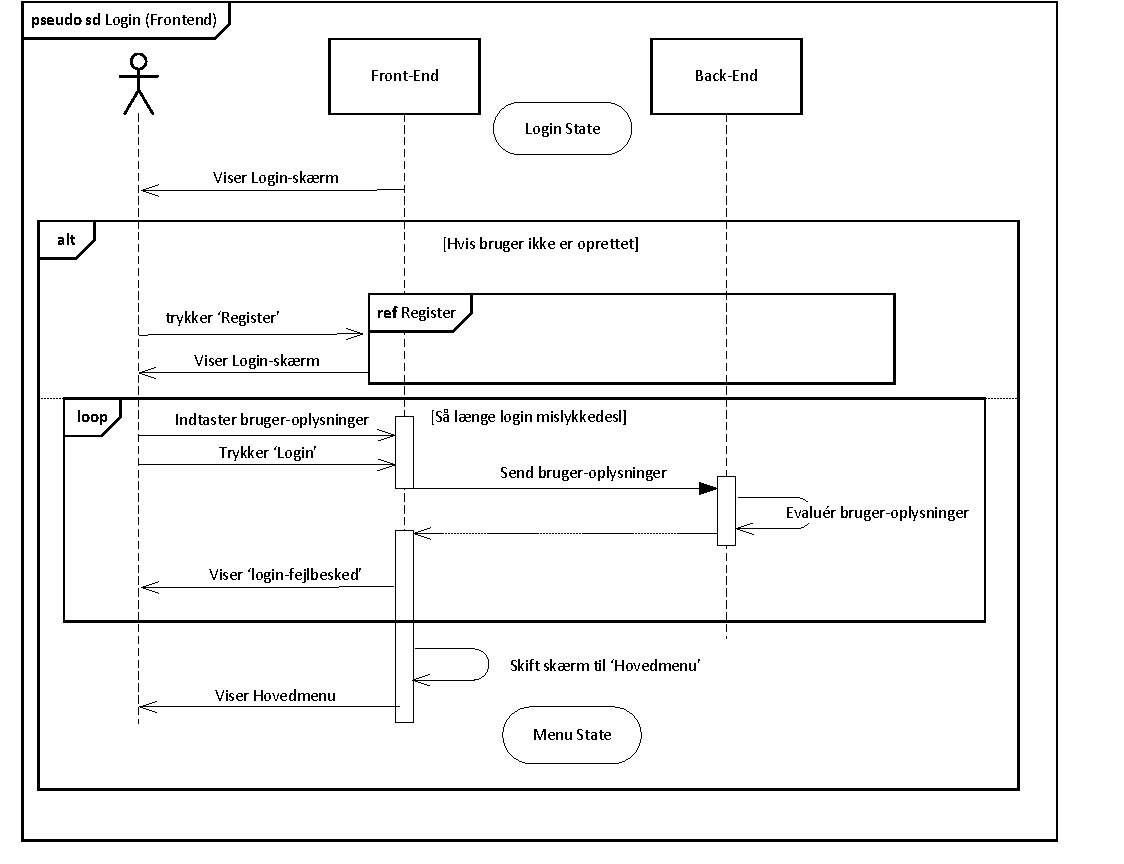
\includegraphics[width = \textwidth]{02-Body/Images/Front-End_-_Arkitektur-login.pdf}
\caption{Pseudo sekvensdiagram af forløbet af userstory "Login", set fra Frontends perspektiv. Med reference til "Register" userstory og håndtering af forkerte login oplysninger.}
\label{fig:Arkitektur-FrontEnd-Login}
\end{figure}

\noindent Dernæst ses "Register" (\autoref{fig:Arkitektur-FrontEnd-Register}), som viser forløbet af hvordan en bruger kan registrere sig med en profil i systememt. Der kan ses på \autoref{fig:Arkitektur-FrontEnd-Login}, at hvis en bruger ikke er oprettet skal man gøre dette først. Derefter skal man vælge et brugernavn og kodeord, hvis brugernavnet er ledigt og alt ellers går godt, kommer man tilbage til "Login" skærmen. ellers får man en fejlbesked på skærmen og bliver bedt om at prøve med et andet brugernavn.\\

\begin{figure}[H]
\centering
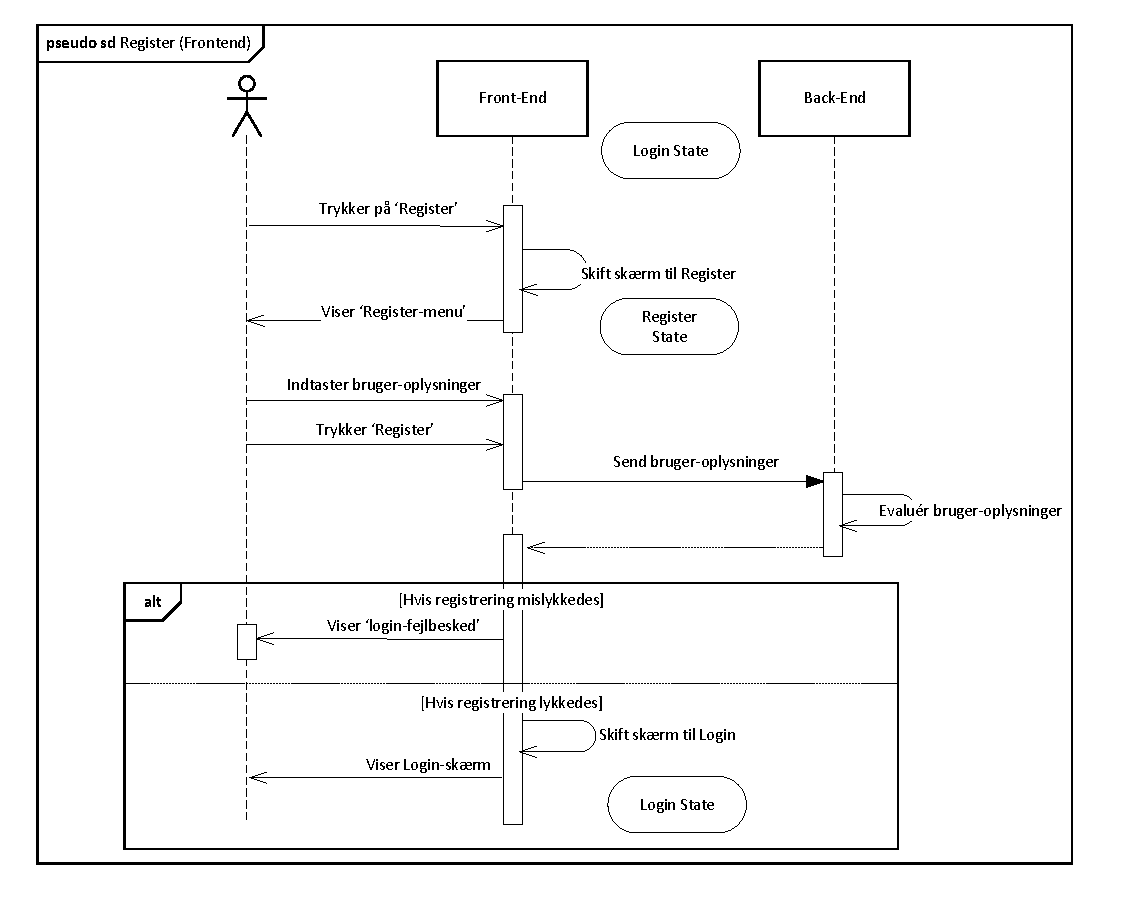
\includegraphics[width = \textwidth]{02-Body/Images/Front-End_-_Arkitektur-register.pdf}
\caption{Pseudo sekvensdiagram af forløbet af userstory "Register", set fra Frontends perspektiv. Med håndtering af forkerte login oplysninger.}
\label{fig:Arkitektur-FrontEnd-Register}
\end{figure}

\noindent På \autoref{fig:Arkitektur-FrontEnd-Save} ses "Save Game", som viser forløbet når en bruger gerne vil gemme sit igangværende spil, set fra Frontends perspektiv. Her kan man bide mærke i, at når der skiftes skærm, vil den nye skærm få initialiseret sine variabler i sin constructor og derfor er der kun et selv kald hver gang skærmen skiftes.
Hertil skal der nævnes at hvis brugeren er i "Combat State" er det ikke muligt at gemme spillet og knappen "Save Game" på "In Game Menu" vil ikke kunne ses eller bruges.\\

\begin{figure}[H]
\centering
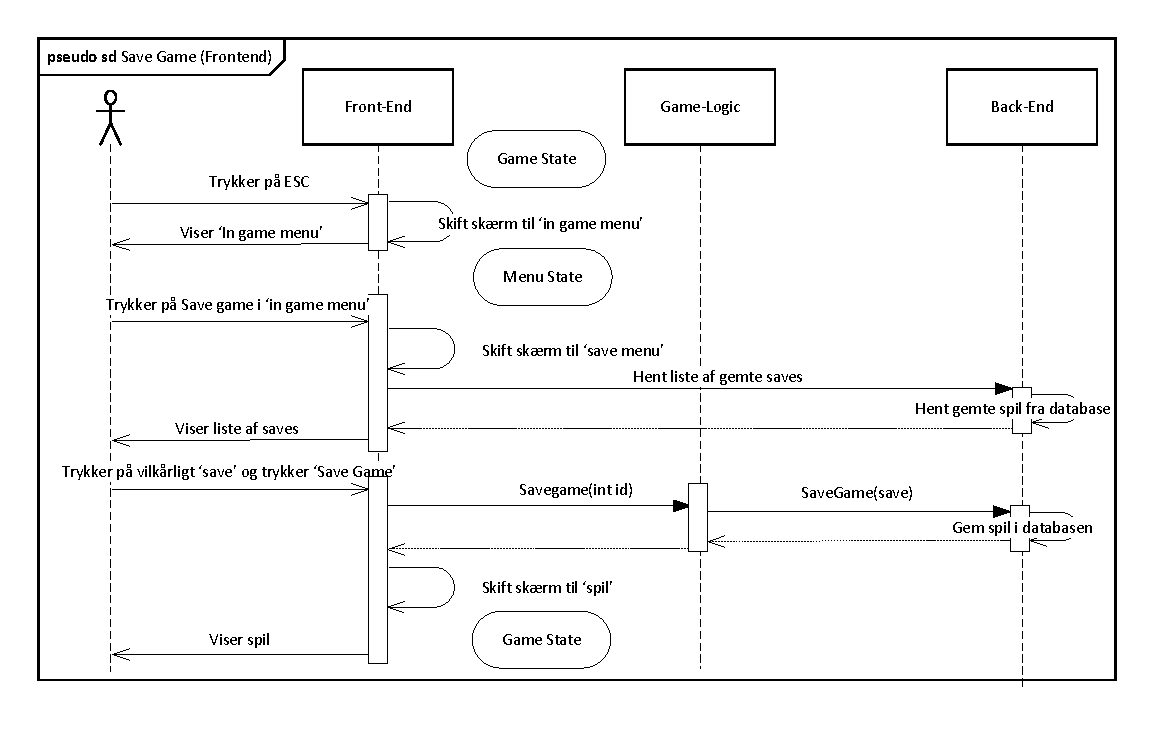
\includegraphics[width = \textwidth]{02-Body/Images/Front-End_-_Arkitektur-savegame.pdf}
\caption{Pseudo sekvensdiagram af forløbet af userstory "Save Game", set fra Frontends perspektiv. Der laves 2 kald til databasen igennem Backenden, hvori der i det første kald,  "Hent liste af gemte saves" hentes en liste af brugerens gemte spil og i andet kald gemmes brugerens nuværende spil henover det valgte spil.}
\label{fig:Arkitektur-FrontEnd-Save}
\end{figure}

\noindent Tilsidst kan der på \autoref{fig:Arkitektur-FrontEnd-Load} ses "Load Game", som viser forløbet når en bruger gerne vil hente et tidligere gemt spil fra databasen, set fra Frontends perspektiv. Denne userstory minder på mange måder om "Save Game", men i stedet for at sende et element til databasen, skal der hentes et gemt spil fra databasen, med alle de data der skal bruges for at kunne loade sit spil op præcis som man forlod det. \\

\begin{figure}[H]
\centering
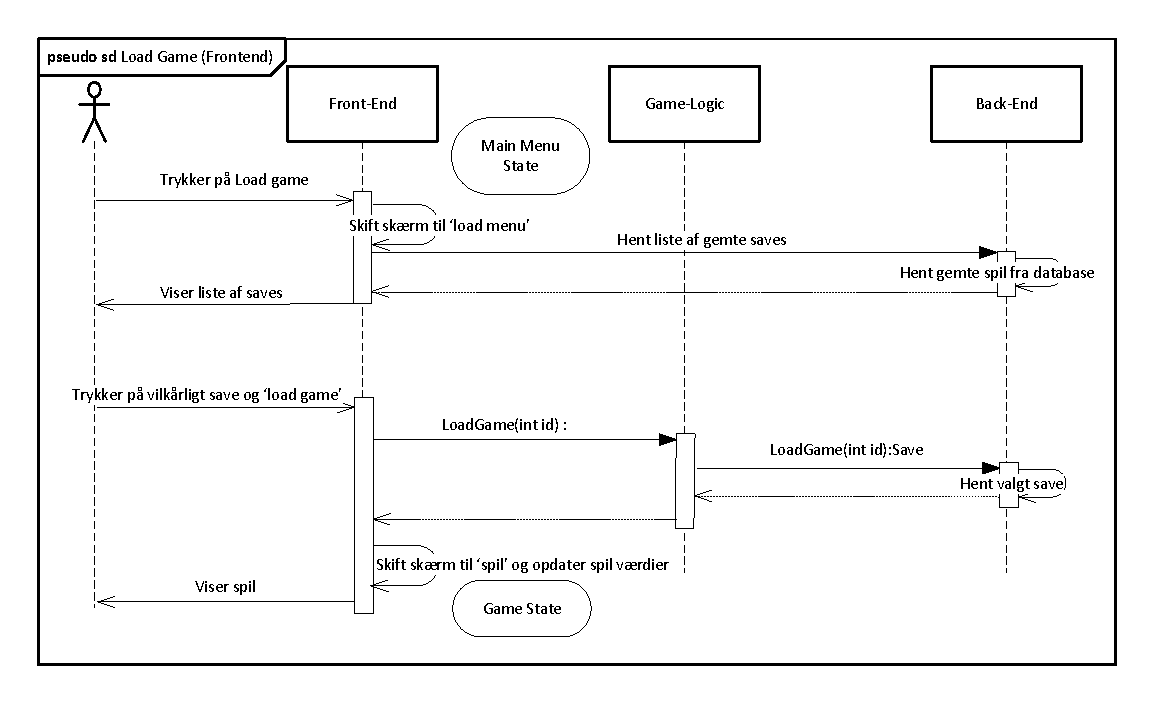
\includegraphics[width = \textwidth]{02-Body/Images/Front-End_-_Arkitektur-loadgame.pdf}
\caption{Pseudo sekvensdiagram af forløbet af userstory "Load Game", set fra Frontends perspektiv. Der laves 2 kald til databasen igennem Backenden, hvori der i det første kald,  "Hent liste af gemte saves" hentes en liste af brugerens gemte spil og i andet kald hentes  brugerens valgte spil og spillet startes op.}
\label{fig:Arkitektur-FrontEnd-Load}
\end{figure}

\newpage

\subsection{GameEngine Arkitektur}
GameEnginens rolle er at skabe logikken for brugeren i spillet. GameEnginens rolle for systemet er afgørende, når spillet er startet for brugeren. GameEnginenens funktionalitet indebærer blandt andet at skabe et map for brugeren, så spilleren kan flytte fra rum til rum ved start af spil. Her forekommer det at brugeren anvender Front End til at interagere med spillet og derefter kan funktionerne fra GameEngineen kaldes.
\subsubsection{States og Character interagering}
\begin{figure}[H]
\centering
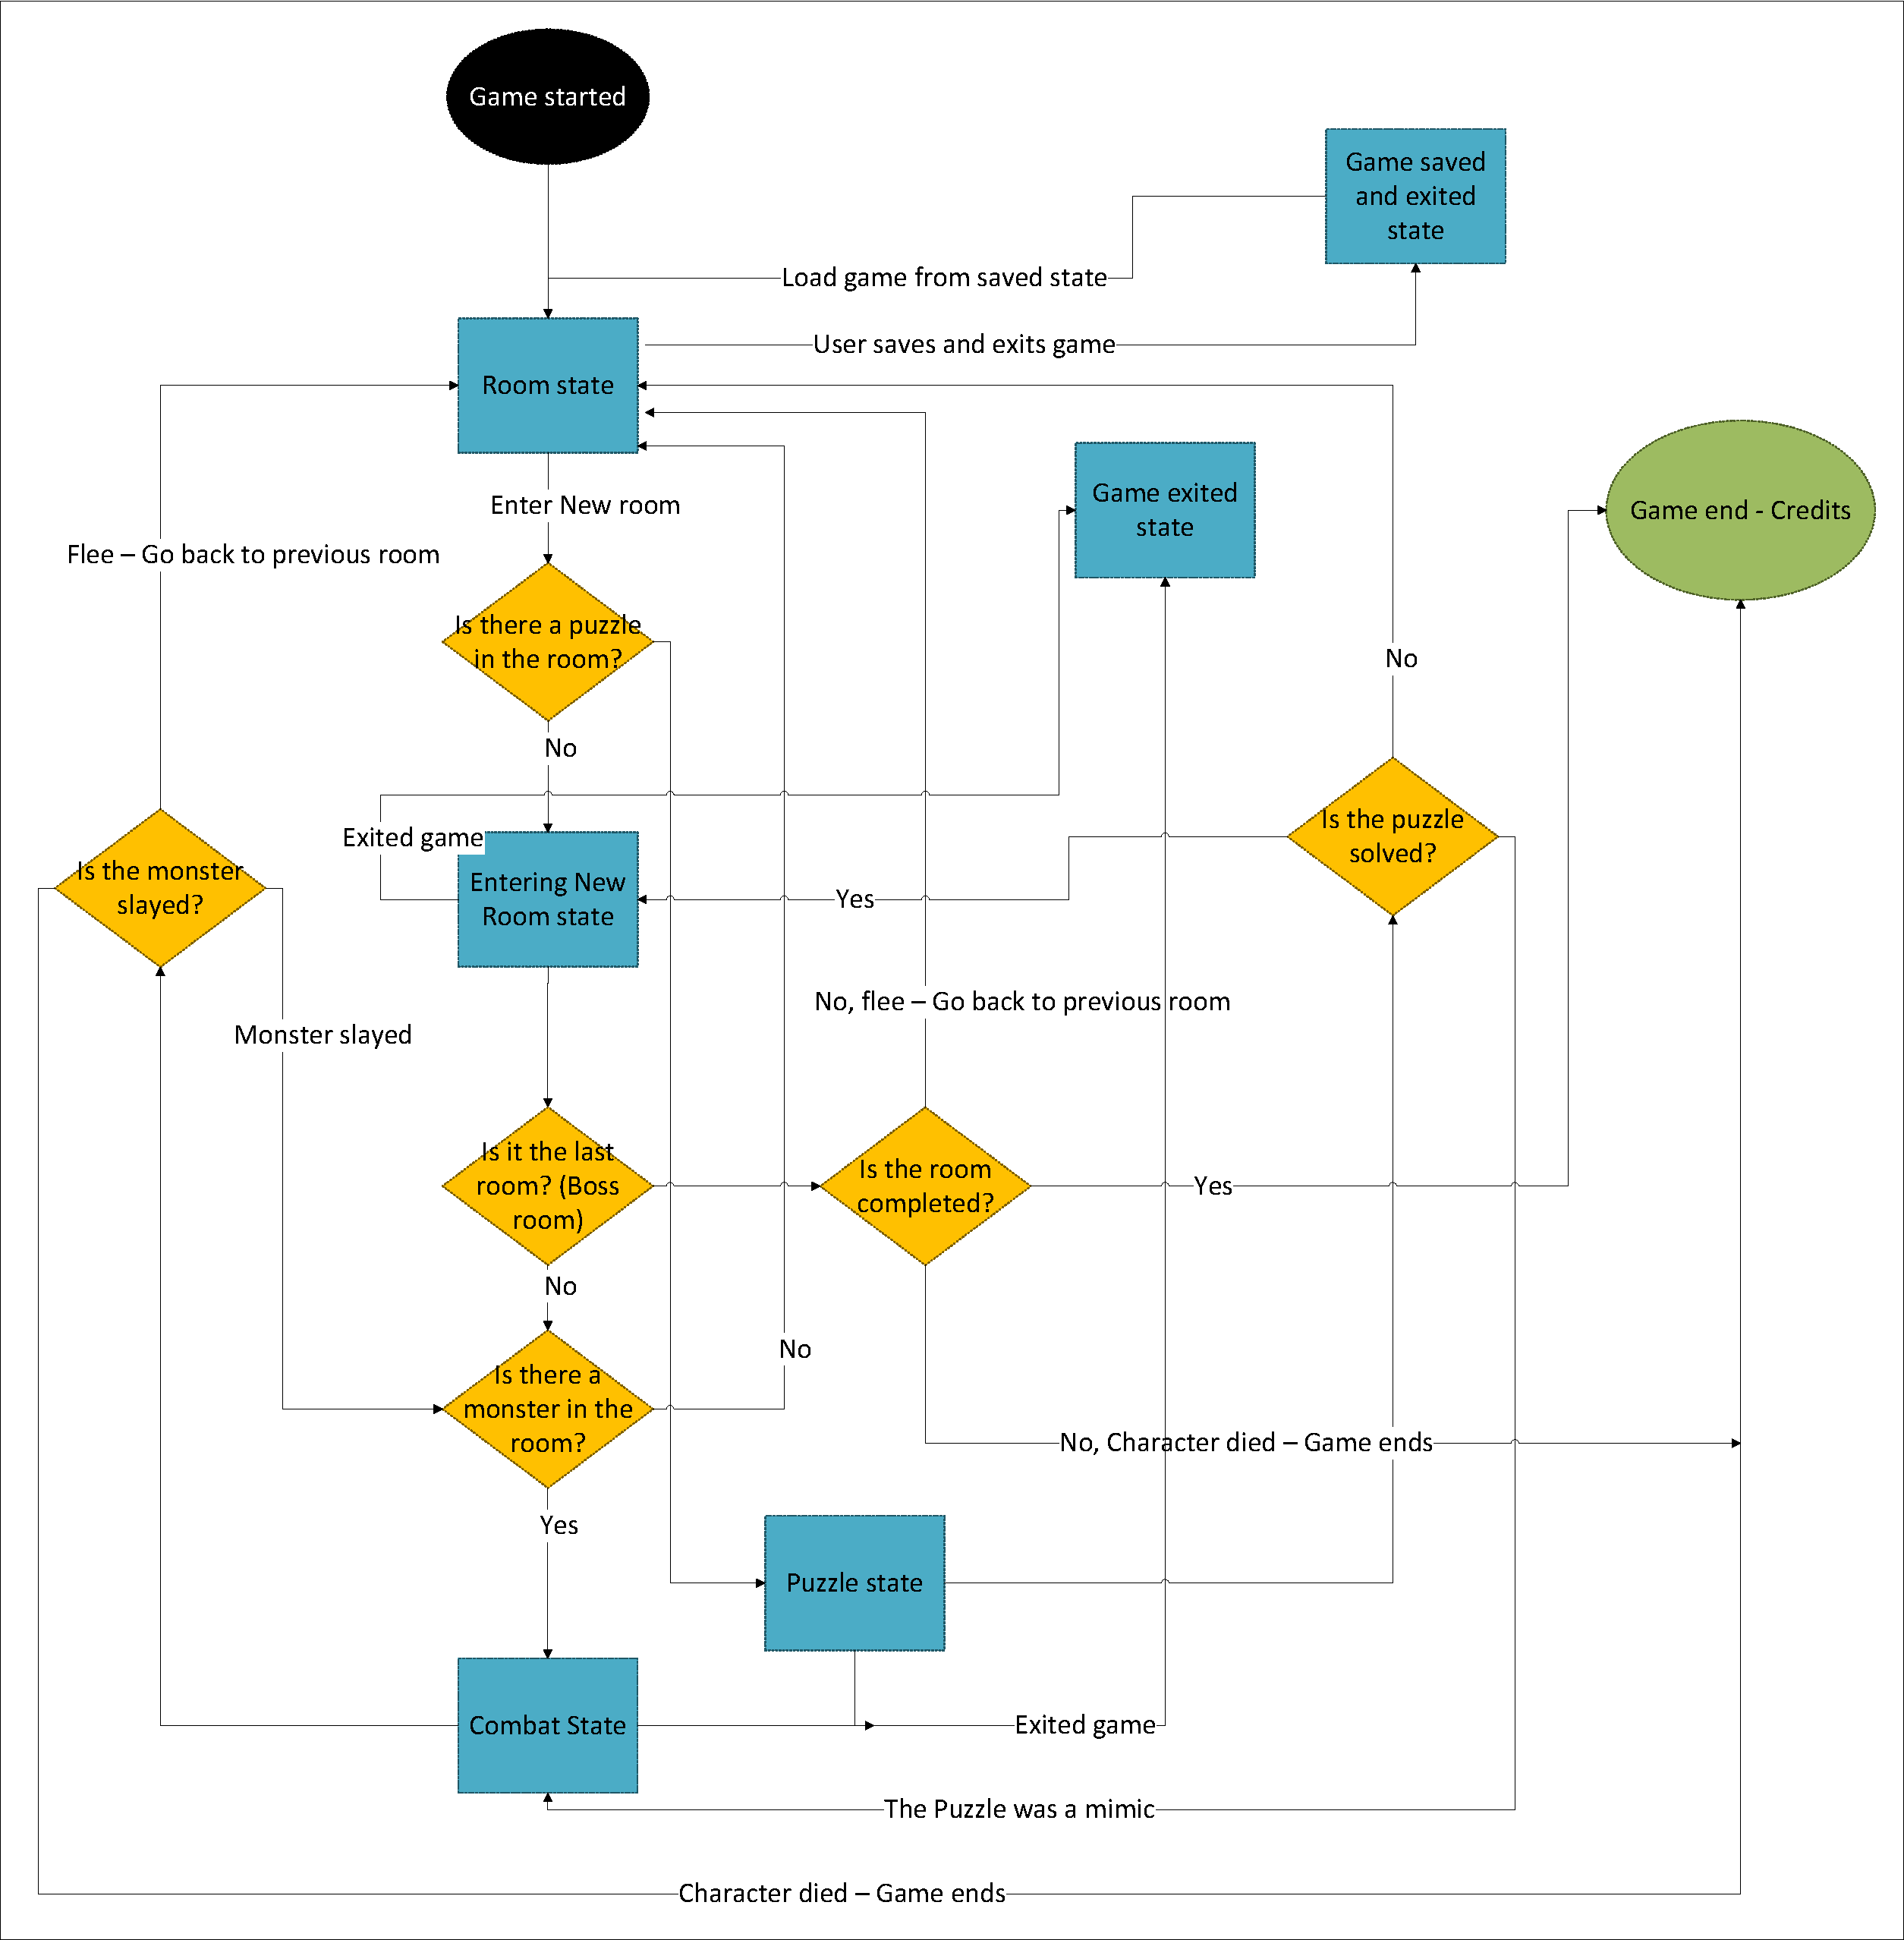
\includegraphics[width = \textwidth]{02-Body/Images/Arkitektur - State Logic.pdf}
\caption{Flow Chart over systemets states når spillet er startet. Dette bilag viser arkitekturen over det ønskede states i systemet når bruger har startet spillet. Dette viser også hvordan spillets fremgang er ønsket og hvordan bruger kommer videre i spillet igennem de forskellige states.}
\label{fig:Arkitektur-SD-SaveGame}
\end{figure}
\subsubsection{Room State og Character interagering}
GameEngineen er delt op i spillets game states som kan ses i bilaget ovenover. Der er hovedsageligt 2 states når spillet er startet. Room State og Combat state. Når spillet er startet for brugeren, starter brugeren i et room state. I dette state kan der interageres med rummet, hvis der er genstande til stede. Her kan brugeren også brugerdefinere sin spiller ved brug af knappen inventory og skifte våben eller skjold. Her kan der også se spillerens evner ved brug af knappen Character. Derudover er der også implementeret beskrivelser fra de forskellige rum som hentes fra modulet Database via modulet Back end.
\subsubsection{Combat State og Combat simulering}
Combat state indebærer når spilleren møder en fjende. Dette sker når man går ind i forskellige rum. Der er oprettet klasser for spillerens evner i form af Attack(Spillerens evne til at slå) og Armor(Spillerens evne til at modstå angreb). Når spilleren angriber en fjende foregår det ved at brugeren trykker på knappen ’Attack’. Når dette forekommer er der implementeret en terning i GameEnginenen. Dette skal implementeres ved to implementeringer. En simuleret terning i form af en pseudo random-number generator som genererer et tal mellem 1 og parameteren numOfSides og en  En Rekursive Psudo-Random number generator som tager en tuple (numOfSides, numOfDice). Den gentager rekursivt implementering 1. Et antal gange svarende til NumOfDice parameteren og summere alle resultaterne.  Hvis brugeren taber kampen, skal brugeren starte et nyt spil eller loade et save. I figuren under ses et Flow chart over forløbet når spiller går ind i combat state.
\begin{figure}[H]
\centering
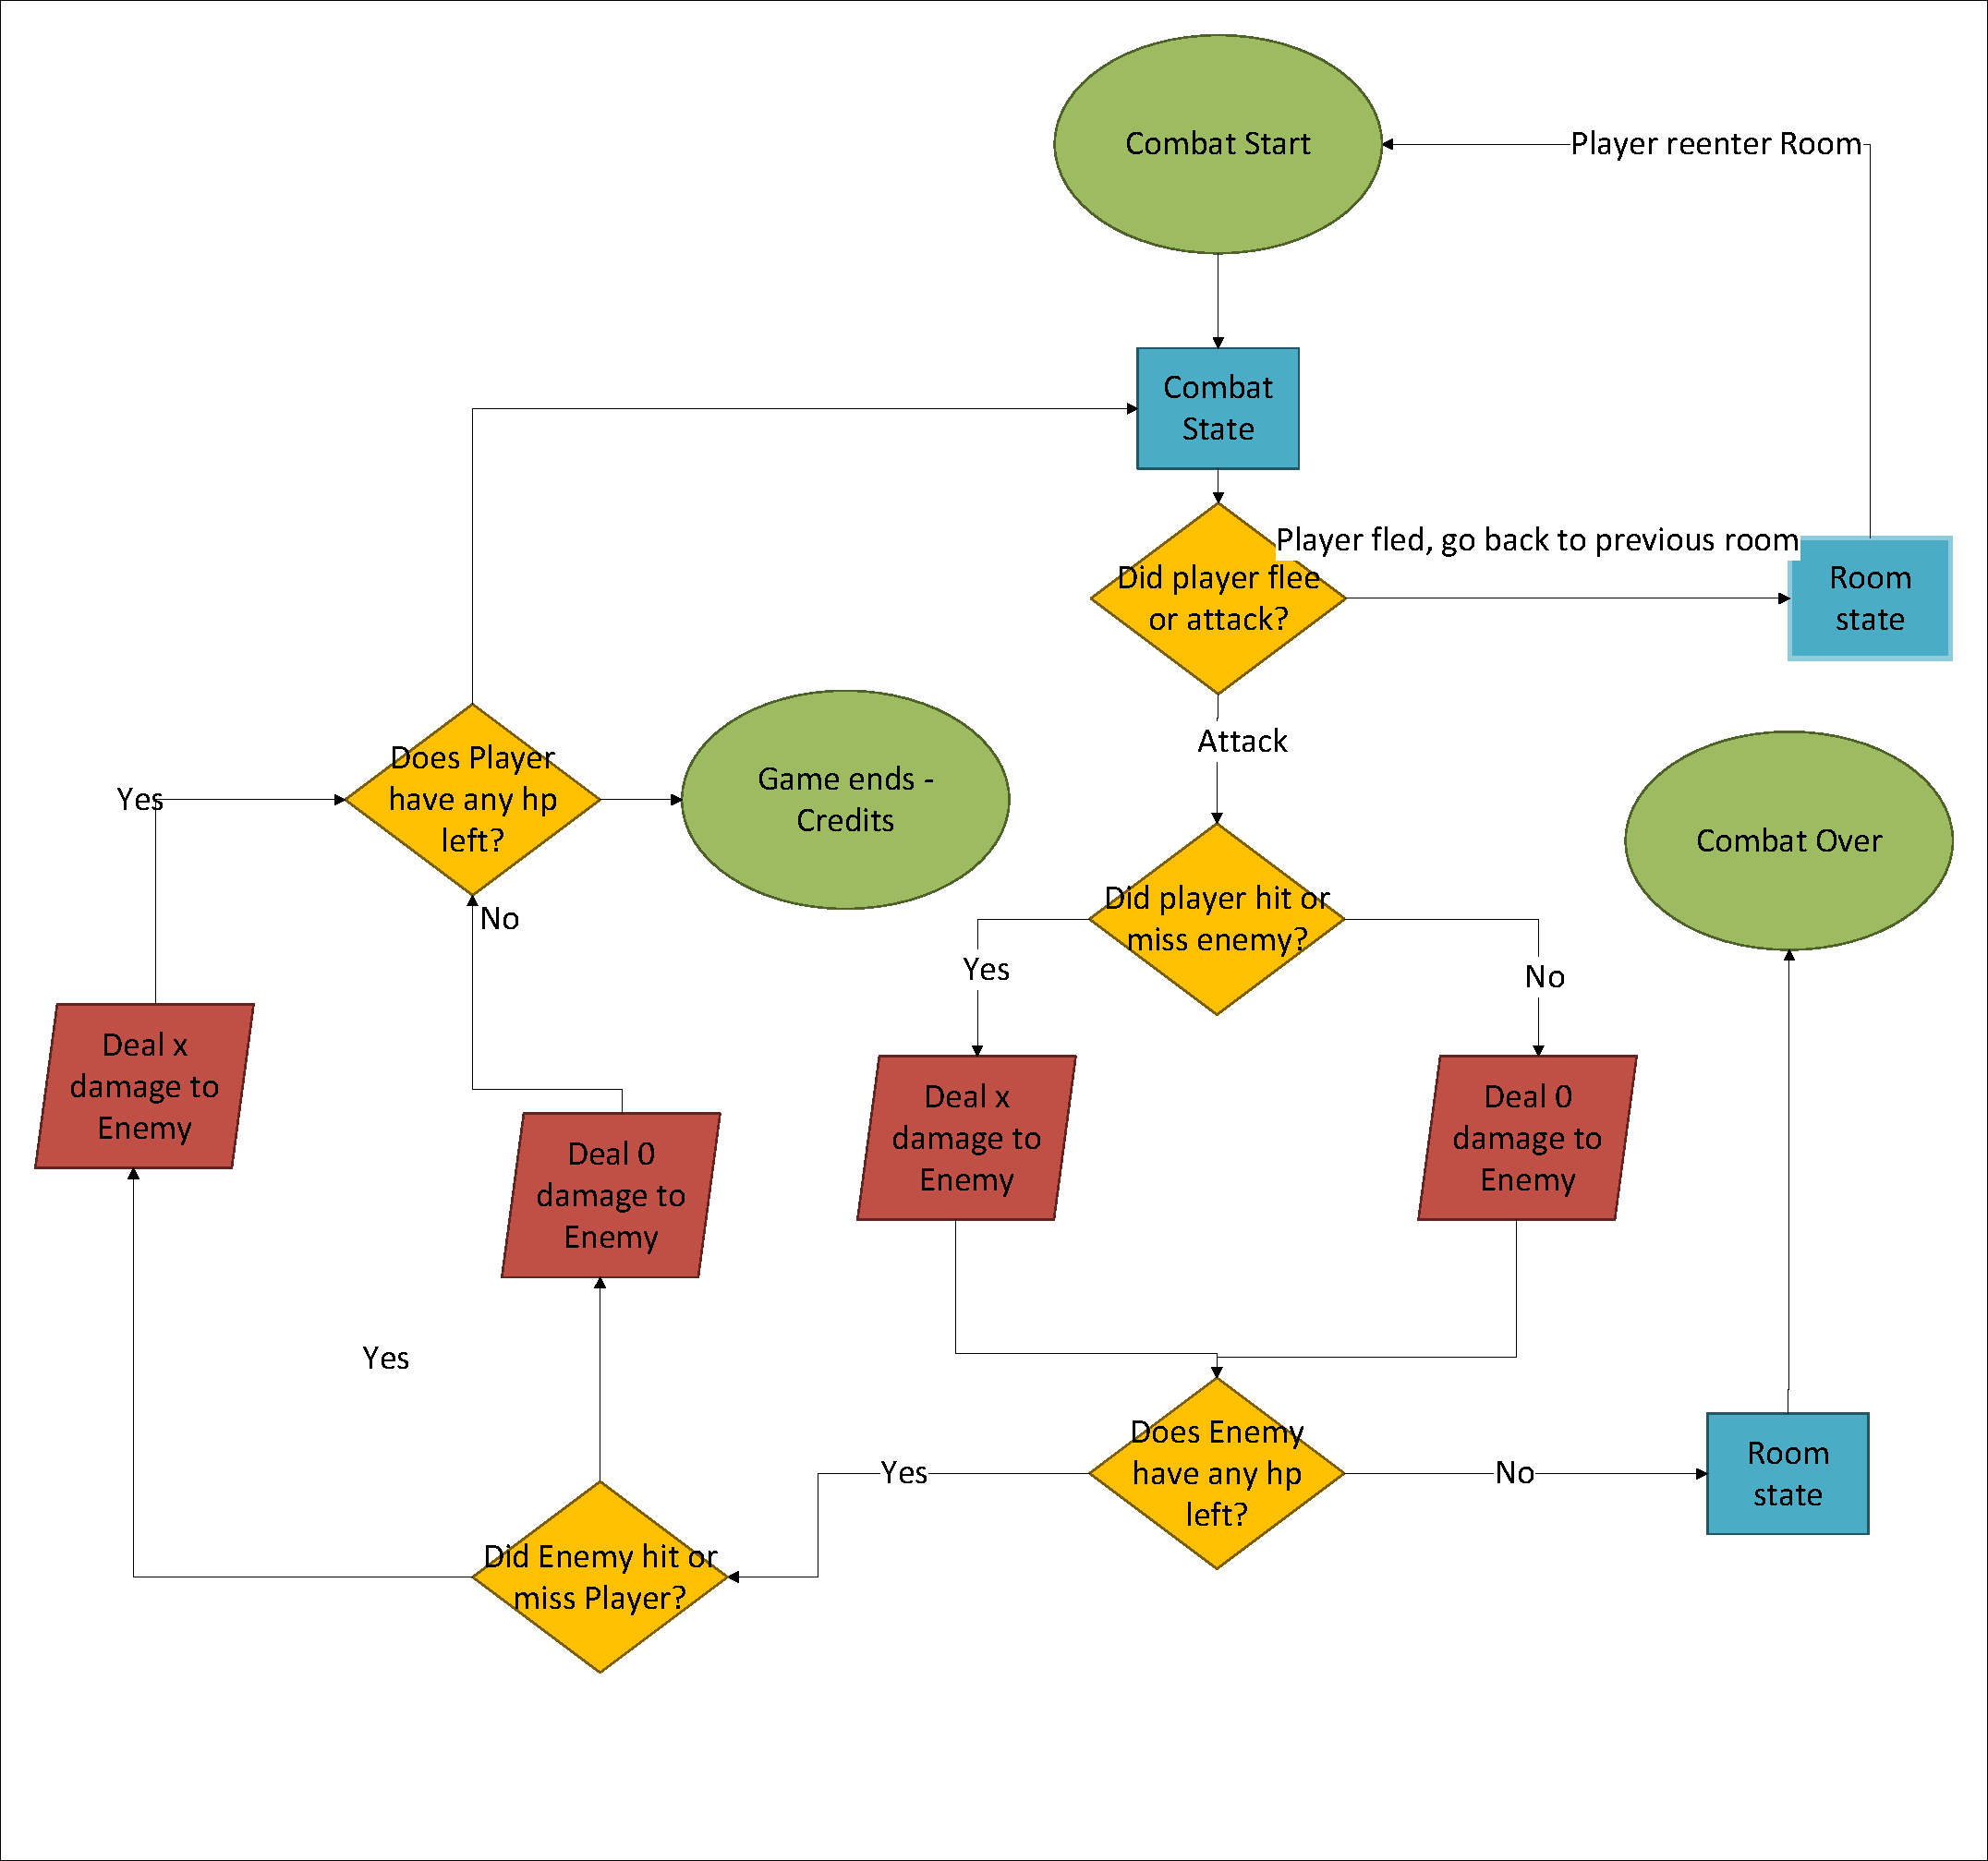
\includegraphics[width = \textwidth]{02-Body/Images/Arkitektur - Combat State.pdf}
\caption{Flow Chart over spillets fremgang når spiller går ind i combat State. Når spiller går ind i et rum med en fjende i rummet, går spillet ind i combat state. Herfra skal spillets terning simulerer et tilfældigt nummer ud fra spilllerens evner. Fjendens evner er bestemt i forvejen. Angreb fastlægges om spiller ruller højere end fjendens Armor Class og vice versa De tre outcomes for spilleren er følgende: Spiller flygter(flee-knap), Spilleren mister alt liv(Spil sluttes) og fjende mister alt liv(Spiller går til room state)}
\label{fig:Arkitektur-SD-SaveGame}
\end{figure}
\subsubsection{Forbindelser til andre moduler}
GameEngineen er forbundet med systemets Back-end og Front-End. Den håndterer data fra Back-end som derefter kan håndteres, så Front-end kan kalde funktionerne fra GameEnginenen. Det data som skal håndteres er primært gemmets forløb som kan lagres i databasen under brugeren. Herefter kan bruger loade det samme gem igen med samme fremgang som da bruger gemte spillet. Det vil være nuværende rum, rum der er blevet besøgt, fjender der er blevet bekæmpet og genstande der er samlet op og taget på.


\subsection{Backend Arkitektur}

I dette afsnit redegøres for arkitekturen af backend containeren. Dokumentet vil først komme med en kort redegørelse for MVC mønstrets opbygning og dets bidrag til arkitekturen. Dernæst gennemgås de relevante krav, hvad angår backenden, disse krav bruges som input til arkitekturen. Med kravene på plads præsenteres et C3 diagram over backend’en, som viser hvordan Web api’et opbygges. Til slut præsenteres REST principper samt hvordan de anvendes.
Systemets backend vil bestå af et Web API udviklet i frameworket ASP.NET Core. Web API’et skal give mulighed for containeren GameEngine at tilgå databasen igennem HTTP request/responses, for at hente og sende den nødvendige data til databasen. Hertil skal backend’en sørger for Authentication og Authorization af de indkommende kald.\\

\subsubsection{MVC}
Selve Web API’ets arkitektur bygges op omkring MVC (Model-View-Controller) mønstret. En illustration af MVC mønstrets struktur kan ses på \autoref{fig:Arkitektur-Backend-MVC} \cite{MVC pattern}.

\begin{figure}[H]
\centering
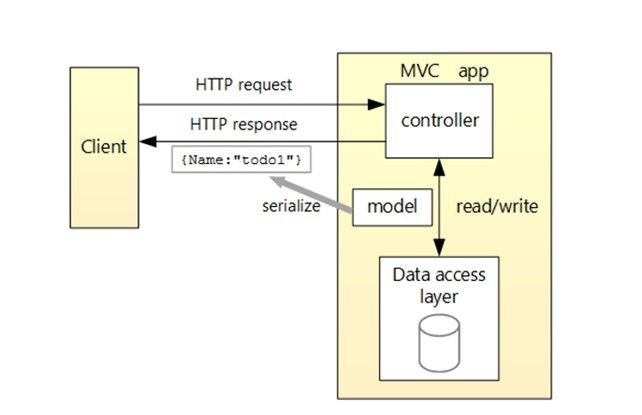
\includegraphics[width = \textwidth]{02-Body/Images/MVC_pattern.JPG}
\caption{Illustration af MVC pattern, bestående af clienter, controller, modeller, og et DAL. som viser hvordan de kommunikerer}
\label{fig:Arkitektur-Backend-MVC}
\end{figure}

Som det kan ses på figuren består mønstret overordnet af 4 dele: client, controller, model og et DAL (Data Access Layer). Da der er tale om et Web API gøres der ikke brug af view moduler. De enkelte moduler har følgende ansvar.

\textbf{Client:}\\
Clientens rolle er at kontakte Web API’et med henblik på at få udført en service, eksempelvis at logge ind.\\
\textbf{Controller:}\\
Controllernes ansvar er at håndterer indkommende kald fra clienten, og route til de rigtige Http endpoints, hvorefter databasen kontaktes igennem DAL.\\
\textbf{DAL:}\\
DAL’s ansvar er at kontakte og administere kommuikation med databasen i form af queries. Det er også her relationerne imellem data objekterne defineres.\\
\textbf{Model:}\\
Modelernes ansvar er at håndtere og definere den data som kan sendes frem og tilbage mellem clienten og databasen, de sørger altså for at binde alle modulerne sammen, således at der er enighed omkring hvordan data objekterne ser ud.\\

\subsubsection{C3-Model for backend}

De relevante user stories for backend containeren udvælges. Disse omhandler håndtering af bruger konti, samt loading og saving af et game state.
 
\begin{itemize}
\item User Story 1 : Log in
\item User Story 2 : Opret Bruger
\item UserStory 7 : Exit Menu -\g Save and Exit
\item UserStory 17 : Main Menu -\g Load List Game
\item UserStory 18 : Main Menu -\g Load Game -\g Load
\item UserStory 19 : Main Menu -\g Load Game -\g Delete Game
\end{itemize}
Af de ikke funktionelle krav er følgende krav relevante:
\begin{itemize}
\item Skal kunne gemme maksimalt 5 save games
\item Skal kunne loade et spil indenfor maksimalt 5 s.
\item Skal kunne respondere indenfor maksimalt 5 s.
\end{itemize}
De ikke funktionelle krav tages hånd om under designet og implementeringen af backenden.
For ydderligere detaljer omkring funktionelle og ikke funktionelle krav henvises til afsnit omkring kravspecifikation \autoref{ssec:Kravspecifikation}


Der bygges videre på C4 modellen for systemet , et level 3 component diagram over backend containeren udarbejdes, som viser hvilke componenter containeren indeholder, deres ansvarsområder, hvordan de kommunikere indbyrdes og med de omkring liggende containere, samt hvilke teknologier der anvendes i implementeringen. Diagrammet kan ses på \autoref{fig:Arkitektur-Backend-C3}. 


\begin{figure}[H]
\centering
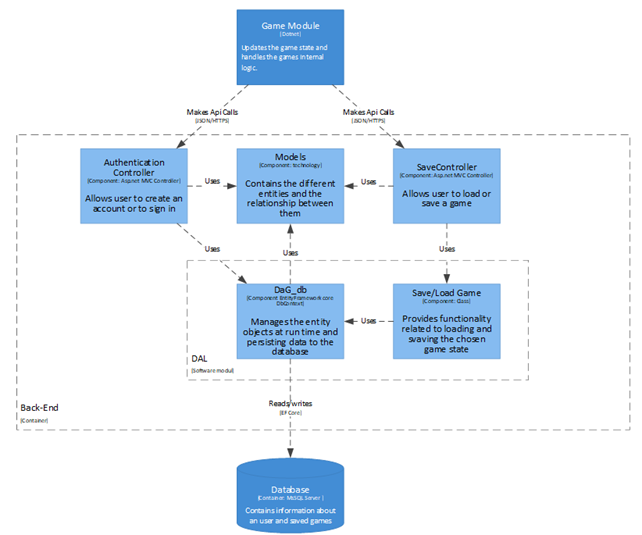
\includegraphics[width = \textwidth]{02-Body/Images/Backend_C3.PNG}
\caption{C3-Model over Backend container,figuren giver et overblik over de componenter backenden består, samt hvordan disse kommunikere indbyrdes og med omkring liggende containere.}
\label{fig:Arkitektur-Backend-C3}
\end{figure}

Figuren illustrerer en lagdelt struktur, hvor der ses en client som kalder ned i controllerne Authentication og Save Controller, som kalder videre til DAL, som så tilgår databasen denne kommunikationsvej går begge veje.

\textbf{Client:}\\
Der eksisterer en client, som kommunikerer med backenden Game Module. Game Module’s kald til backenden kan overordnet set indeles i to undergrupper, bruger håndtering og save håndtering. Bruger håndtering indeholder kald som omhandler login og registreing  (User story 1 og 2), hvor save håndtering omhandler loading og saving af Game state (User story 7, 17, 18 og 19). Kommuniaktionen her vil foregå ved netværkskald med protokolen HTTPS. Clienten udfører request/response kald til backenden igennem specifikke URL’s. For at data objekterne kan sendes frem og tilbage med HTTPS kæves disse seralizeres og deseralizeres mellem JSON-objekter og .Net objekter.\\
\textbf{Controller:}\\
Inde i backenden anvendes ASP. Net MVC controllere(Mangler ref) til at modtage og svare på kald fra clienten. Der laves en controller for Bruger håndtering og en controller for Save håndtering. Hver request mappes til en specifik controller. Controllerne vil så indeholde action metoder, som udføres når den modtagere et kald. Når controlleren har udført sin action retuneres et Action Result, hvor i et data objekt kan wrappes eller den kan indeholde en fejlmeddelse hvis noget går galt.\\
\textbf{DAL:}\\
De to controllere kalder som sagt videre ned i DAL laget, dette lag består af en database kontekst DaG\_db og en hjælper klasse til at udfører Queries. Her gøres brug af EF (Entity Framework) Core, som gør det muligt at arbejde med DbContext klassen, denne bruges til skabe en kontekst af databasen, hvor i de enkelte modeller kan mappes til entities.\\

\textbf{Model:}\\
Modellerne fungerer som bindeledet mellem alle komponenterne, de definerer den data som der arbejdes på, og vil blot bestå af en række C\# klasser.\\

Som det kan ses passer MVC mønstret perfekt til den funktionalitet der ønskes. Mønstret gør det muligt at lave en logisk gruppering af relaterede opgaver, og er med til at sikre høj samhørighed i applikationen, ved at de enkelte ansvarsområder fordeles ud på hver sine moduler. På figur 1 \autoref{fig:Arkitektur-Backend-C3} ses det tydeligt hvordan koblingen mellem de enkelte moduler holdes på et lavt niveau, hvilket gør det lettere at bygge videre på og tilføje ny funktionalitet.\\


\subsubsection{REST}
Web Api’et arkitektur vil gøre brug af REST principper, for ikke at gøre data overførelserne for komplekse og for at overholde SoC, ved at adskille repræsentationen og dataen fra hinanden. På den måde sikres det at dataen, kan blive repræsenteret på den ønskede måde, og ikke er tvunget til at blive gemt på en specifikt måde.
Dette kommer til udtryk ved følgende 5 REST principper(Mangler ref)  som søges opnået:
\begin{enumerate}
 \item Alle de data objekter der arbejdes med tilhører en bestemt unique URI. Dataen hentes, sendes og manipuleres igennem standard HTTP metoder som (GET, POST, PUT, DELETE).
 \item Der arbejdes ud fra en client/server arkitektur med data som resource. 
 \item Web Api’et er stateless, hvilket vil sige der gemmes ikke nogen tilstand omkring clienten på server siden.
 \item Der arbejdes ud fra en lagdelt struktur, som betyder at hver component kun kan se de componenter som grænser op til den selv.
 \item Der anvendes Cashing på server siden (Dette vil ikke blive implementeret).
\end{enumerate}

\subsubsection{Konlusion}

Systemets backend består at Web Api, som bygges op omkring MVC mønstret, som gør det muligt at lave en logsik gruppering af den enkelte funktionalitet. Web Api’et vil ligeledes gøre brug af REST principper for at adskille data resourcerne fra deres repræsentation på clientens side.

\newpage

\subsection{Database Arkitektur}

I oprettelsen af systemets database skal der tages hånd om, hvordan kommunikationen skal foregå imellem systemets segmenter, samt databasens funktionalitet. Her er der blevet besluttet at der anvendes en DAL, der fungerer ved at hver gang databasen skal kontaktes, så foregår det igennem denne. Yderligere vil denne DAL også simplificere kommunikationen mellem databasen og Back-End.

\begin{figure}[H]
\centering
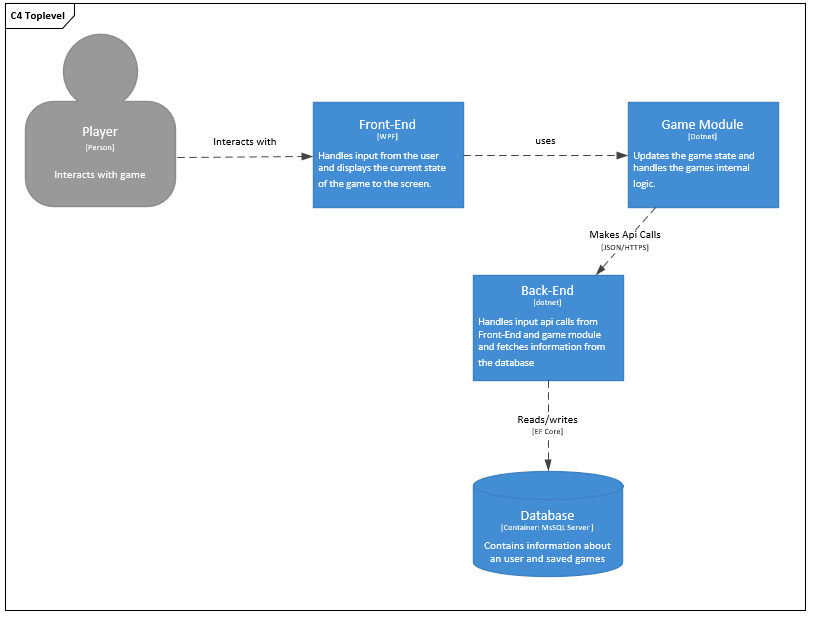
\includegraphics[width = \textwidth]{02-Body/Images/C4TopLvlDB}
\caption{C4 top level diagram, som viser kommunikation mellem systemets segmenter}
\label{fig:C4TopLvlDB}
\end{figure}

Måden kommunikationen vil foregå igennem systemet vises her. Her ses der at en bruger interagere med Front-End, data går videre til Game Module, som kommunikere med Back-End, hvor der til sidst enten bliver skrevet til databasen eller hentet data fra databasen
For at illustrere databasens funktionalitet er der blevet dannet sekvensdiagrammer, som viser hvordan databasen vil kunne gemme et spil og hente et gemt spil.

\begin{figure}[H]
\centering
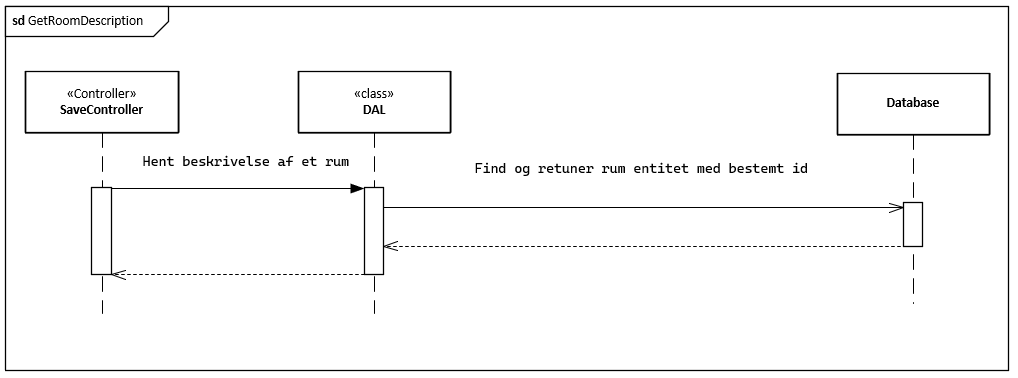
\includegraphics[width = \textwidth]{02-Body/Images/RoomDescriptionsDB.PNG}
\caption{Sekvensdiagram for hvordan rum beskrivelser vil blive hente fra databasen af SaveController}
\label{fig:RoomDescriptionsDB}
\end{figure}

I diagrammet GetRoomDescription ses der, hvordan kommunikationen ville foregå for at hente rum beskrivelsen. Her ses der at SaveController, fra Back-End, går til DAL, som så henter rum beskrivelsen fra databasen, og herefter returneres dataene fra databasen til DAL og så fra DAL til SaveController.

\begin{figure}[H]
\centering
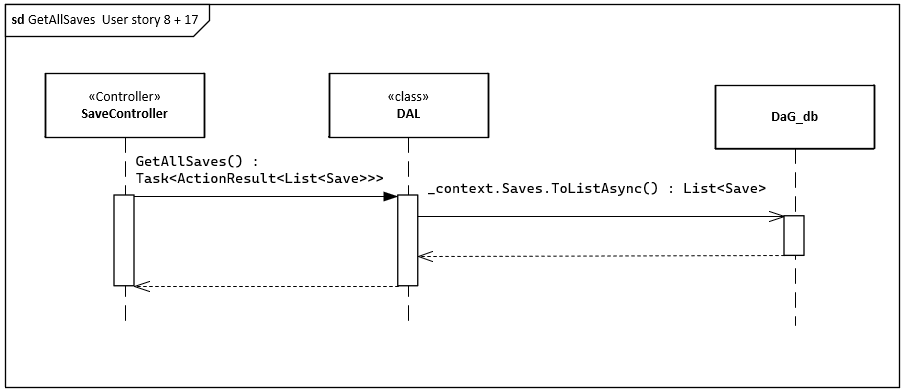
\includegraphics[width = \textwidth]{02-Body/Images/GetAllSavesDB.PNG}
\caption{Sekvensdiagram for User story 17: GetAllSaves, i relation til hentet data fra database}
\label{fig:GetAllSavesDB}
\end{figure}

I diagrammet GetAllSaves foregår kommunikation på samme måde som ved at hente rum beskrivelser. Forskellen her er dog at der i stedet for hentes en list af alle gemte spil.

\begin{figure}[H]
\centering
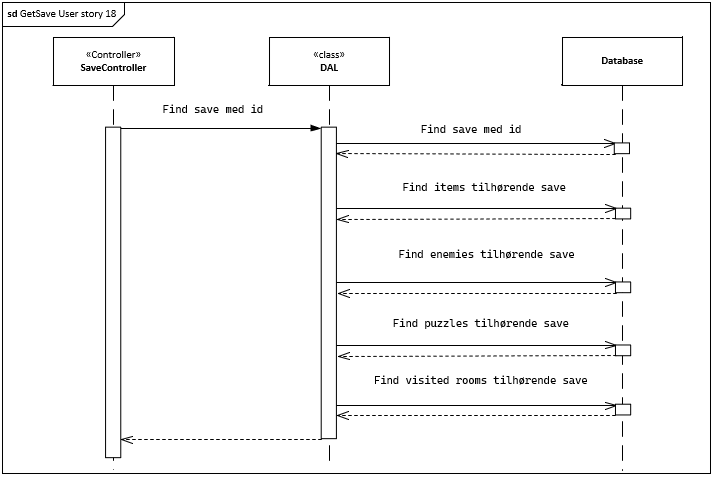
\includegraphics[width = \textwidth]{02-Body/Images/GetSaveDB.PNG}
\caption{Sekvensdiagram for User story 18: GetAllSaves, i relation til hentet data fra specifikt gemt spil fra database}
\label{fig:GetSaveDB}
\end{figure}

I diagrammet GetSave ses der hvordan et specifikt gemt spil hentes. Her ses der at dataene igen går først igennem DAL. Et gemt spil vil have et ID, som der kan anvendes til at finde de korresponderende værdier som dette gemte spil har. Her ses der at der vil findes items, enemies, puzzles og hvilke rum en spiller har besøgt. Dataene returneres herefter til DAL og så til SaveController.

\begin{figure}[H]
\centering
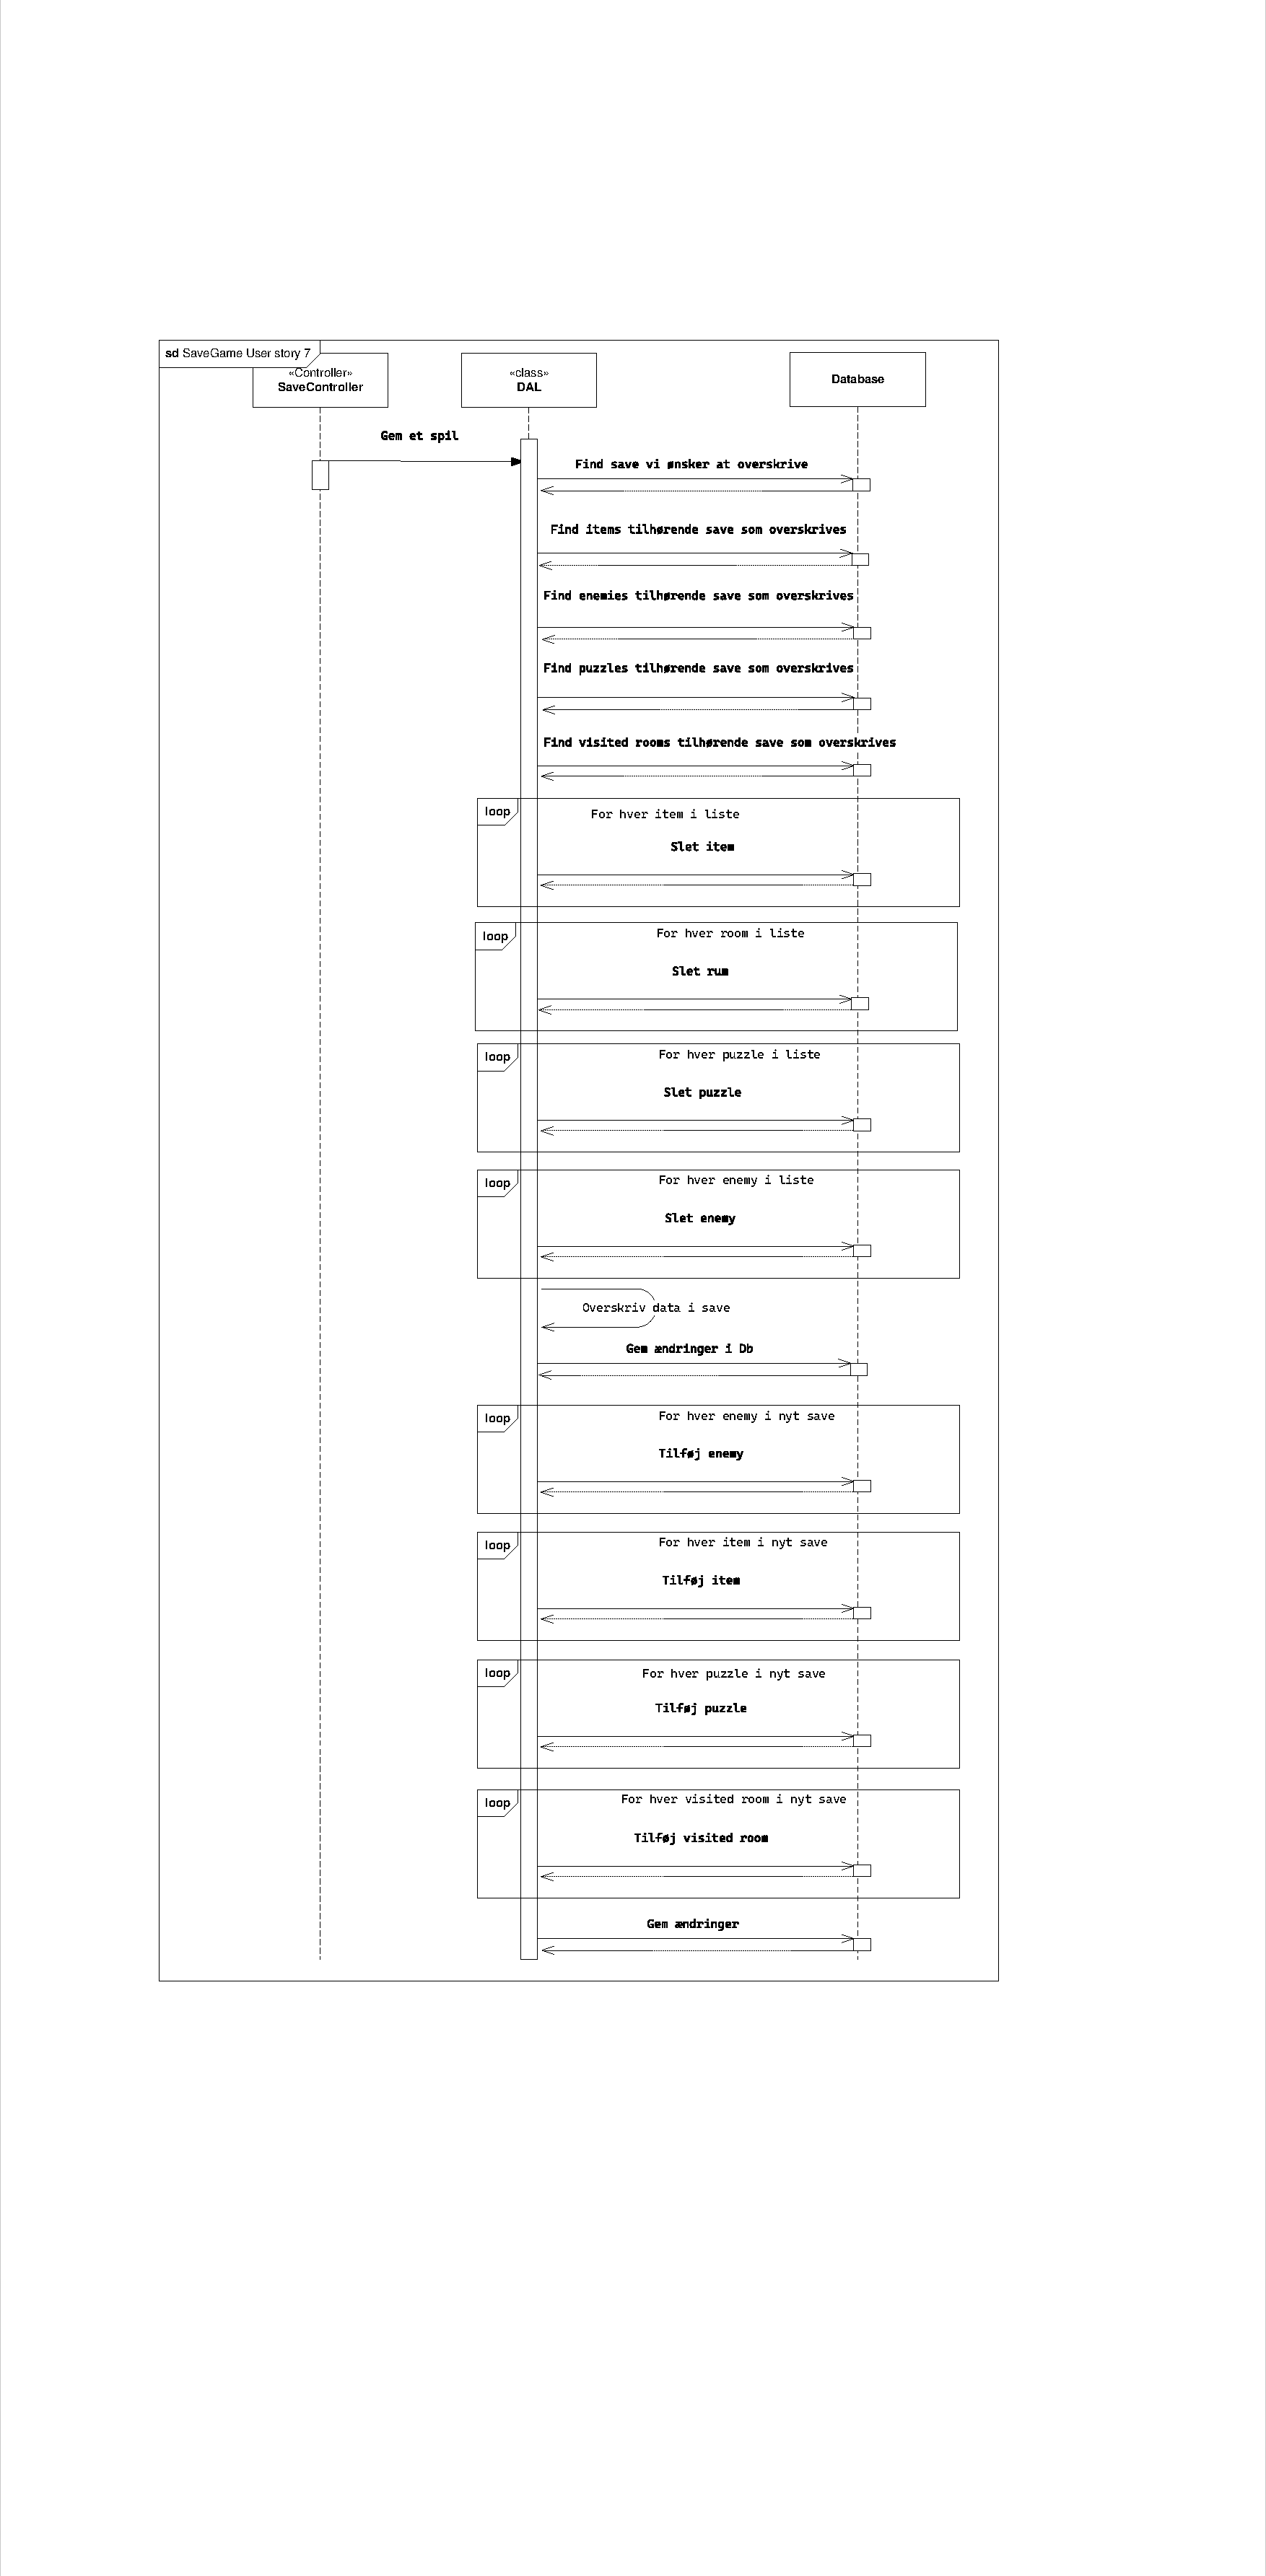
\includegraphics[width = \textwidth]{02-Body/Images/SaveGameDB.pdf}
\caption{Sekvensdiagram for User story 7: SaveGame. Dette diagram viser hvordan et spil gemmes}
\label{fig:SaveGameDB}
\end{figure}

I dette diagram, SaveGame, ses der hvordan et spil vil gemmes. Måden dette vil fungere på er at spilleren vil starte med fem tomme gemte spil, som bliver seeded til databasen. Dette bliver gjort for at begrænse en bruger til fem gemte spil. Så for at gemme et spil findes der først hvilket gemte spil der skal overskrives. Derefter findes de relevante værdier i dette gemte spil. Hernæst slettes disse værdier og der tilføjes de nye korrekte værdier.\\
Brugeren vil derfor ikke have mulighed for at oprette et nyt spil, men kun mulighed for at overskrive en af fem tomme spil, som bliver oprettet for hver bruger.



\subsection{DAL Arkitektur}
I dette segment vil der blive forklaret tankerne bag arkitekturen vedr. oprettelsen af en funktionel DAL, som kan anvendes til at styre kommunikationen til og fra databasen.
Til oprettelsen af en funktionsdygtig database, i dette projekt, kræves der et relativt tæt sammenhold mellem databasen og backend api’en. API’en er ansvarlig for kommunikation mellem Front-end, Game Module og databasen.

\begin{figure}[H]
\centering
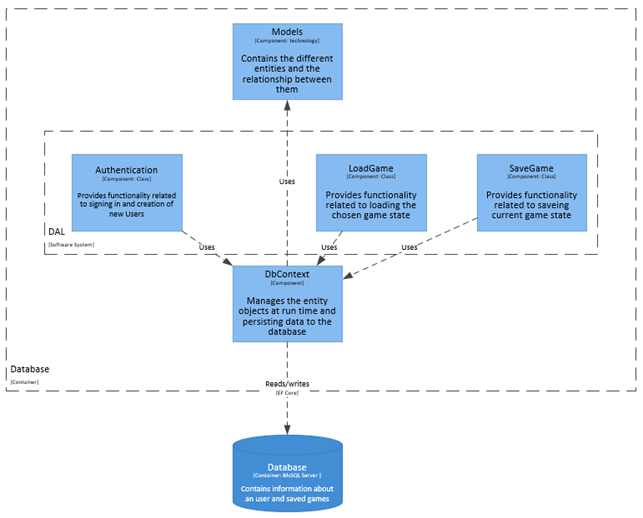
\includegraphics[width = \textwidth]{02-Body/Images/DALArkitektur}
\caption{C3 diagram for blokkene involveret i DAL's funktionalitet}
\label{fig:DALArkitektur}
\end{figure}


Når data enten skal sendes til eller hentes fra databasen så er det igennem et DAL. Systemets DAL giver os en simplificeret adgang til dataene gemt i databasen, og fungerer som en mellemmand for systemet, da alt kommunikation til databasen går igennem den.
I denne DAL har vi en Authentication, som bliver anvendt når en bruger logger ind, og når der oprettes en ny bruger. Denne blok kontrollerer brugernavn og kodeord, som sendes og hentes i databasen. Ydermere vil der ikke sættes fokus på sikkerhed, som ses i kravene stillet for systemet.
Yderligere vil det også være muligt at både gemme et spil og indlæse et spil. Begge af disse vil operere på det samme data, dog ville den ene, LoadGame, hente data fra systemets database, og den anden, SaveGame, vil sende data til systemets database. 
LoadGame i DAL er ansvarlig for at hente spillerens data fra databasen, såsom hvilket rum de var i og mængden af liv de har tilbage. 
Hernæst er der SaveGame. Denne indeholder funktionaliteten for at sende et gemt spil, altså dataene for spillerens nuværende spil. Heri vil der også gemmes information og spillerens nuværende tilstand i spillet. Det ville f.eks. være rummet som spilleren er i når spillet bliver gemt.
Begge af disse vil være ansvarlige for at håndtere data som er individuelle for hver spiller og hvert gemt spil.
Udenfor systemets DAL ville der også være inkluderet Models i konstruktionen af systemets database. Models vil indeholde de entities som Authentication og Load-/SaveGame vil bestå af. Yderligere vil Models også være ansvarlig for forholdene imellem de forskellige entities. 



\begin{figure}[H]
\centering
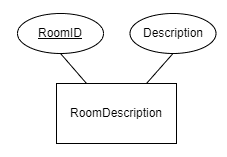
\includegraphics[width = \textwidth]{02-Body/Images/ER-RoomDescription.PNG}
\caption{ER diagram for Roomdescription. En beskrivelse består blot af en beskrivende string samt det tilhørende unikke rumid.}
\label{fig:ER-Roomdescription}
\end{figure}

